%%%%%%%%%%%%%%%%%%%%%%%%%%%%%%%%%%%%%%%%%%%%%%%%%%%%%%%%%%%%%%%%%%%%%%
% Lớp 9 | Chương V. Đường tròn | Cung và dây của một đường tròn
% Dạng 9H5?14-1: Quan hệ giữa đường kính và dây
%%%%%%%%%%%%%%%%%%%%%%%%%%%%%%%%%%%%%%%%%%%%%%%%%%%%%%%%%%%%%%%%%%%%%%


% nguồn: dan_tu_AI (nhập 14/11/2026)
\begin{ex}%[9H5N14-1]%[ma:4f99efd5]
	Cho đường tròn $(O;6\text{ cm})$. Dây dài nhất của đường tròn này có độ dài là
	\choice
	{$6\text{ cm}$}
	{$3\text{ cm}$}
	{\True $12\text{ cm}$}
	{$36\text{ cm}$}
	\loigiai{
		Đường kính là dây lớn nhất của đường tròn, có độ dài $2R=12\text{ cm}$.
	}
\end{ex}

% nguồn: dan_tu_AI (nhập 14/11/2026)
\begin{ex}%[9H5H14-1]%[ma:11986902]
	\immini{Cho đường tròn $(O;10\text{ cm})$ và dây $AB=12\text{ cm}$. Đường kính $CD$ vuông góc với $AB$ tại $H$, $H$ nằm giữa $O$ và $D$ (như hình bên). Độ dài đoạn thẳng $CH$ là}
	{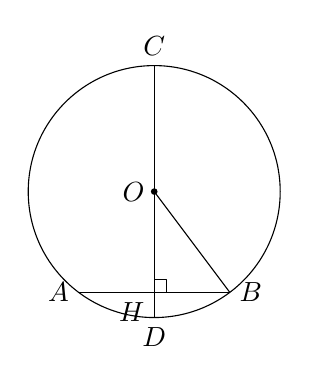
\begin{tikzpicture}[scale=0.8,line join=round]
		\draw (0,0) circle (2);
		\draw (0,2)--(0,-2);
		\draw (-1.2,-1.6)--(1.2,-1.6);
		\draw (0,0)--(1.2,-1.6);
		\draw (0,-1.6) rectangle (0.2,-1.4);
		\fill (0,0) circle (1.5pt);
		\node[left] at (0,0) {$O$};
		\node[above] at (0,2) {$C$};
		\node[below] at (0,-2) {$D$};
		\node[left] at (-1.2,-1.6) {$A$};
		\node[right] at (1.2,-1.6) {$B$};
		\node[below left] at (0,-1.6) {$H$};
	\end{tikzpicture}}
	\choice
	{$2\text{ cm}$}
	{\True $18\text{ cm}$}
	{$16\text{ cm}$}
	{$14\text{ cm}$}
	\loigiai{
		Tam giác $OAB$ cân tại $O$ ($OA=OB$) có $OH$ là đường cao nên cũng là đường trung tuyến, suy ra $HB=\dfrac{AB}{2}=6\text{ (cm)}$.\\
		Tam giác $OHB$ vuông tại $H$: $OH=\sqrt{OB^2-HB^2}=\sqrt{100-36}=8\text{ (cm)}$.\\
		Vì $H$ nằm giữa $O$ và $D$ nên $CH=CO+OH=10+8=18\text{ (cm)}$.
	}
\end{ex}

% nguồn: dan_tu_AI (nhập 14/11/2026)
\begin{bt}%[9H5V14-1]%[ma:d8ddb64a]
	\immini{Một ống nước có mặt cắt là hình tròn bán kính $50\text{ cm}$. Mặt nước trong ống (theo mặt cắt) là dây $AB$ rộng $80\text{ cm}$ và mặt nước thấp hơn tâm $O$ của ống (như hình bên). Tính chiều sâu lớn nhất của nước trong ống (đơn vị: cm).}
	{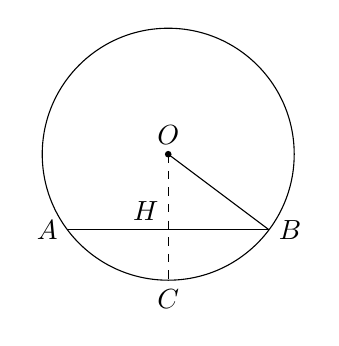
\begin{tikzpicture}[scale=0.8,line join=round]
		\draw (0,0) circle (2);
		\draw (-1.6,-1.2)--(1.6,-1.2);
		\draw[dashed] (0,0)--(0,-2);
		\draw (0,0)--(1.6,-1.2);
		\fill (0,0) circle (1.5pt);
		\node[above] at (0,0) {$O$};
		\node[left] at (-1.6,-1.2) {$A$};
		\node[right] at (1.6,-1.2) {$B$};
		\node[above left] at (0,-1.2) {$H$};
		\node[below] at (0,-2) {$C$};
	\end{tikzpicture}}
	\shortans{20}
	\loigiai{
		Kẻ đường kính qua $O$ vuông góc với $AB$ tại $H$, cắt đường tròn tại $C$ (phía dưới).\\
		Tam giác $OAB$ cân tại $O$ nên $H$ là trung điểm $AB$, $HB=40\text{ cm}$.\\
		$OH=\sqrt{OB^2-HB^2}=\sqrt{2500-1600}=30\text{ (cm)}$.\\
		Chiều sâu lớn nhất: $HC=OC-OH=50-30=20\text{ (cm)}$.
	}
\end{bt}
